%% ****************************************************************
%% Document type and general settings
%% ****************************************************************

\documentclass[11pt,a4paper,oneside,bibtotocnumbered,pointlessnumbers,liststotoc]{scrbook}%

%% ****************************************************************
%% Packages
%% ****************************************************************

\usepackage[dvips]{graphicx}
\DeclareGraphicsExtensions{.eps}
\DeclareGraphicsRule{.eps.gz}{eps}{.eps.bb}{'zcat #1}
\renewcommand\floatpagefraction{.9}
\renewcommand\topfraction{.9}
\renewcommand\bottomfraction{.9}
\renewcommand\textfraction{.1}   
\setcounter{totalnumber}{50}
\setcounter{topnumber}{50}
\setcounter{bottomnumber}{50}

\usepackage{blindtext}

\usepackage{ee2}               
\usepackage{amsmath}                           
\usepackage[amssymb]{SIunits}  
\usepackage[intoc]{nomencl}   
\usepackage{multirow}             
\usepackage{multicol}
\usepackage{tabularx}         
\usepackage{acronym}
\usepackage[table]{xcolor}	% changing rowcolors
\usepackage{longtable}	%tables over multible pages
\usepackage[latin1]{inputenc}       
\usepackage[T1]{fontenc}                             
\usepackage{caption} 
\usepackage[german, english]{babel}					
\usepackage[]{epsfig}
\usepackage{subfig}
\usepackage{setspace}
\usepackage{geometry}
\usepackage[headsepline]{scrpage2}
\usepackage{verbatim}           
\usepackage{hvfloat}	%rotating tables and pictures
\usepackage{subfloat}
\usepackage{enumitem}
\usepackage{here}
\usepackage[default,oldstyle,scale=0.95]{opensans} 


\usepackage[pdftitle={Title}, pdfauthor={Autor}, bookmarks=true, pdfborder={0 0 0}]{hyperref}


\usepackage[
	style=ee2,
	citestyle=authoryear,
	firstinits=true,
	backend=bibtex
	]{biblatex}
\addbibresource{literature.bib}

%% ******************************************************************
%% Page and font settings
%% ******************************************************************


\renewcommand{\baselinestretch}{1.5}%     % Zeilenabstand
\geometry{a4paper, left=30mm, right=20mm, top= 20mm, bottom=20mm, headsep=5mm, footskip=5mm}%
\setlength{\parindent}{0em}%           
\setlength{\parskip}{0ex}%

\setcounter{secnumdepth}{3}
\setcounter{tocdepth}{3}

\setkomafont{title}{}
\setkomafont{chapter}{\Large}
\setkomafont{section}{\large}
\setkomafont{subsection}{}
\setkomafont{subsubsection}{} 
\setkomafont{paragraph}{} 
\setlist[description]{%
  font={\bfseries}, % set the label font
}


\setkomafont{chapterentry}{\textbf}
\renewcommand*{\chapterheadstartvskip}{\vspace*{0mm}}

\pagestyle{scrheadings}
\clearscrheadfoot
\ohead{\headmark}
\ofoot[\pagemark]{\pagemark}

\makenomenclature

%% ********************************************************************************
%% Main document
%% ********************************************************************************

\begin{document}

%% Frontmatter
\frontmatter
%\include{Chapters/title_page1}  

\titlepage{
\vspace*{10mm}
	\center{

		\Large{

    	\begin{figure}[h]
      	\begin{center}
      	\includegraphics*[width=8cm]{Pictures/TU_Logo_SW.pdf}
      	\end{center}
    	\end{figure}

			\vspace{5mm}

			Seminar Paper} \\

	\vspace{6mm}

%%% Title

	\Large{\textbf{Modeling of Oil Market
\\}}

	\vspace{15mm}
Technische Universit{\"a}t Dresden\\
    Chair of Energy Economics\\
    Prof. Dr. Dominik M{\"o}st\\
\vspace{9mm}
    \begin{figure}[!htb]
      \begin{center}
      \includegraphics*[width=2.5cm]{Pictures/ee2_Logo_2020.png}
      \end{center}
    \end{figure}
\vspace{5mm}
	
%%% Information about the group and group members
	
	\normalsize{\textbf{Group \#Modeling of oil market}\\
							Course of Stuides: Literature Studies of topics of interest in Energy Economics\\
							\vspace{6mm}
	    				Academic Supervisor: Matthew Schmidt\\}

	\vspace{8mm}
	Date of Submission: 31.07.2020 \\
  \vspace{30mm}
  }
  }
\newpage
\thispagestyle{empty}

\vspace*{\fill}
\begin{center}
\Large{\textbf{Group 4}}\\

\vspace{10mm}

\normalsize{
\textbf{Yushan Yang}\\
yushan.yang@mailbox.tu-dresden.de\\
Matricul. No.: 4874821\\

\vspace{5mm}

\textbf{Yu Kong}\\
yu.kong@mailbox.tu-dresden.de\\
Matricul. No.: 4899848\\

\vspace{5mm}

\textbf{Xiao Cui}\\
xiao.cui@mailbox.tu-dresden.de\\
Matricul. No.: 38150815\\			

\vspace{5mm}

\textbf{Dongxin Guo}\\
dongxin.guo@mailbox.tu-dresden.de\\
Matricul. No.: 4825168\\			

\vspace{5mm}

\textbf{Anurag Trivedi}\\
anurag.trivedi@mailbox.tu-dresden.de\\
Matricul. No.: 4821519 \\
}							
\end{center}
\vfill
	% for group work

\pagenumbering{Roman}
\setcounter{page}{1}

\chapter*{Abstract}

Volatility in the oil market affects macroeconomic conditions.  Oil market modeling provides a framework for understanding oil market trend. In recent years, the world oil market is becoming more and more complex. And new methods are needed to perceive, simulate, and predict today's oil market. This review introduces several research and literature about the model of the oil market in world oil market, and divides these studies and methods into three categories: structural models, reduced form models, and artificial intelligence models. In structural model we focus on game-theoretical model, optimization model and simulation model. This classification is used to study the advantages of each method and limitations, to provide guidance for future researchers to select appropriate models for oil market modeling.
\tableofcontents
%\listoffigures				% not needed for seminar papers
%\listoftables				% not needed for seminar papers
%\printnomenclature		% not needed for seminar papers

%% Content
\mainmatter
\pagenumbering{arabic}


\chapter{Introduction}
Oil is an important commodity in the global economy and an important part of the economic development of industrialized and developing countries. In recent years, the world oil market is becoming more and more complex. Political events, extreme weather, financial market speculation, etc. can all affect the oil market and increase the price volatility of the oil market.

This survey focuses on the models used in the oil market. We discusses the method of constructing the model. We also analyze the advantages and disadvantages of each model by applying the model to oil price prediction and provides guidance for future research or oil market modeling.


Based on the characteristics of the model, we divided these models into three kinds: structural models, reduced form models, and artificial intelligence models. These classifications are not to establish a classification method but to facilitate comparison of the characteristics of the model. Although sometimes there is more than one method when modeling.

Section 2 is a historical analysis of oil price developments. In section 3 we introduced the modeling methods of three major models. In section 3.1, we divided structured models into three categories, optimization models, simulation models, and game theory models. Structural models provide an explanation for the long-term fluctuations in oil prices, but sometimes we want to track short-term oil price trends without having to consider market behavior in detail. Structural models usually refer to too many model parameters. Therefore, compared with structural models, in section 3.2 we introduced the reduced form. It focus on statistical relationships of oil prices and the time changes. Since artificial intelligence models have been increasingly used in oil market models in recent years, and this has become a trend in future modeling, we introduced artificial intelligence models in 3.3. Artificial neural networks differs from these traditional modeling methods by using parametric methods to build models to solve complex structural and nonlinear and dynamic problems. In section 4, we compare these models and discuss their respective advantages and limitations.



\chapter{Oil History}

Petroleum is a commodity which its price follows the law of supply-demand. However, as one of the important strategic materials, there are many factors affecting international oil prices. 
Although supply and demand are the basic determinants, it was also largely influenced by the international economy, political, diplomatic, and military influences, as well as the speculation of the hot money around the world. These influencing factors have effect on short-term oil prices, therefore these long and short term fluctuations in oil prices make it difficult to predict. In this chapter, we will follow the Fig \ref{oilPrice} and briefly introduce the oil price history and the factors affecting it.

\begin{figure}[h]
    \centering
    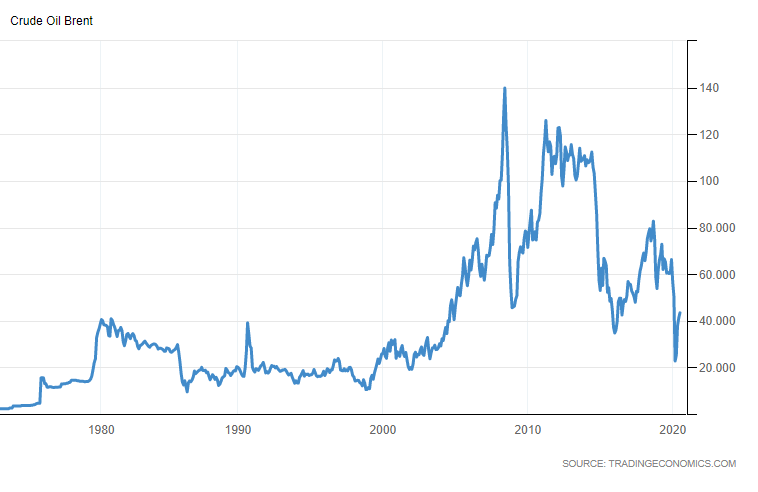
\includegraphics[width=12cm]{template_latex/Pictures/oil_brent.png}
    \caption{Oil price chart (\cite{brent})}
    \label{oilPrice}
\end{figure}

Before the establishment of OPEC in 1960, the oil price was monopolized by the western countries. After 1960, OPEC continuously struggled with Western multinational companies around the production and pricing power of oil.

In 1970s, with a series of victories of OPEC in negotiations, OPEC started to gain the power of the decision of the crude oil price. And the price started to rise at this period. The fourth Middle East war broke out in 1973 and resulted in the price increasing approximately 400\% to \$11 per barrel and the first energy crisis in Western countries. In February 1974, Nixon proposed to hold a meeting between oil-consuming countries then the International Energy Agency (IEA) was established. Energy supply issues have become a priority concern for governments. At the same time, the first modeling project leaded by U.S. government was created. Then a algorithm called "Project Independence Evaluation System (PIES)" (\cite{hogan1975energy}), and it was used for analysts to predict and develop strategies. From 1974 to 1978, crude oil prices remained at 
a certain level of \$11-\$14 per barrel. From 1979 to 1981, the second oil crisis doubled the oil price to the maximum price \$40 per barrel. These two crisis provided motivations for researchers to explore the oil market and subsequently a large amount of oil models were developed. The rising of OPEC's position changed the oil market structure as well as a lot of structural theories related with OPEC were also proposed in researchers' study. 
Later OPEC used the production quota in this period, the price of Brent oil fell slowly from US\$36.83 per barrel to US\$27.51 per barrel.
Then with the growth of crude oil production in non-OPEC oil-producing countries, the development of energy conservation technology and alternative energy sources. OPEC's ability to control oil prices had continued to decline, along with the fall of crude oil prices. In 1986, oil prices fell sharply to around \$10 per barrel. Subsequently the market power started to affect the oil price remains at a level of \$14.3-\$20 per barrel until 1997 except the short-term increase caused by the Gulf War between 1990 and 1991. As a result of the Asian financial crisis, demand decrease, and OPEC's untimely increase in production, the oil price dropped to around \$10 per barrel in 1998. 

Since then the price started to bounce and tripped the price in 18 months and continued to rise after 2003. The financial market began to gradually reflect its role in influencing short-term oil prices (\cite{huntington2013oil}). After reaching the nearly \$140 per barrel in 2008, the price fell sharply to \$45 at the end of the year with the broke out of the global financial crisis. From 2014-2016, the revolution of shale oil shocked the crude oil market. OPEC refused to reduce the production for defending the market share. From June 2014 to January 2016, the price of Brent crude oil fell from the \$115.06 to \$34 per barrel. The trade dispute between China and the United States in 2018 caused the price to fell from the highest price of \$82 to around \$53 per barrel. And then the Coronavirus in 2019 caused the reduction of the demand, with the oil price war between Russian and Saudi-Arabia in 2020 caused the Brent oil price to continue to drop in Spring 2020. The lowest price is \$22 on April 20, even the West Texas Intermediate (WTI) appeared negative price as the reason for that most May 2020 WTI oil futures contract holders could not store the oil as the contract was going to expired.

In recent years, the great development of the computer and the mathematical technology enables researchers to develop modeling systems with massive computing ability. Meanwhile, more historical and reliable data source are accessible. So more and more oil market models were generated compared with the past.

\chapter{Taxonomy of oil market models}

\section{Structural models}

\subsection{Game-theoretic equilibrium models}
Game-theoretic equilibrium model is a kind of structural model. The structural model is based on microeconomic theories. It studies the commodities, the different actors and their interactions in the markets. In the game-theoretic equilibrium model, more than two optimizing agents will be considered, such as OPEC members and non-OPEC producers who want to improve their profits as much as possible. OPEC plays an important role in the oil market, it accounts for 38\% of the world oil production by 2019. It leads the oil market and determines the oil price according to certain rules. Non-OPEC producers are the price-takers in the oil market, most of them can only respond to price changes passively. Demand in this model is usually considered as aggregated global demand which is generally related to GDP and oil price. As the game-theoretic equilibrium does not provide enough computational support, the complexity of different oil will be reduced. Several game-theoretic equilibrium models will be introduced below.
\subsubsection{Nash-Cournot Model}
Salant proposed a model which integrates the theory of exhaustible resources and theory of oligopoly. The hotelling's theory is the fundamental concept for the price prediction for the non-renewable resources. The Nash-Cournot approach allows non-cooperative participants to compete in the oil market where consumers buy the oil at the same price. The cartel starts to form when an individual participant owning more than one firms or plants. The equilibrium will be reached if none of the dominant extractor or competitive fringe are able to solely change their strategies to gain more profit in the market (\cite{salant1976exhaustible}). 

Supposing the marginal cost in the model is constant, which means the cost of each extraction unit is equal no matter how much oil has been extracted. To maximize the discounted revenue, the cartel need to choose a right sales path. As the demand curve and the sales path of the competitive sectors are known, the cartel can get the excess demand by deducting the given sales. Then the cartel need to take account of the marginal revenue to achieve the maximum profit without exceeding its inventory. Here, an equation (\cite{salant1976exhaustible})is introduced:
\[M=P(Q^m+ Q^c )-Q^m\boldsymbol{\cdot}a(P)\] 

$M$ stands for the marginal revenue, $P$ for the price, $Q^m$ for the sales of cartel, $Q^c$ for the sales of the competitive fringe, $a(P)$ for the absolute value of the slope of the demand curve. The equilibrium price path requires that marginal revenue will grow at the rate of interest but will never exceed the rate of interest before the cartel sells out its inventory. As the competitive sector includes speculators who will buy and sell in the periods, they will enter the market as the prices rises to make more profit. When the price increases at the rate of interest, the competitive sector will hold the inventory. Once the price rises at a smaller rate, they will sell the inventory eventually. Supposing both sectors start with a positive inventory, the competitive fringe will first sell the oil out and leave the market to the cartel. The price at this point is denoted with $P*$. Before the time point, both the cartel and competitive fringe exist. Before the price reaches $P*$, it increases at the rate of interest. When the price reaches $P*$, the cartel will take over the market. The marginal revenue will still rise at the rate of interest until the demand is satisfied. The price for the point is denoted as $F$. As is shown in the figure, during the period of $S+T$, both the cartel and the competitors will sell out their inventory, but the competitors sell the oil out during the first period $T$. As long as the price equilibrium exists, the price path will present like Figure \ref{nash1} below.
\begin{figure}[h]
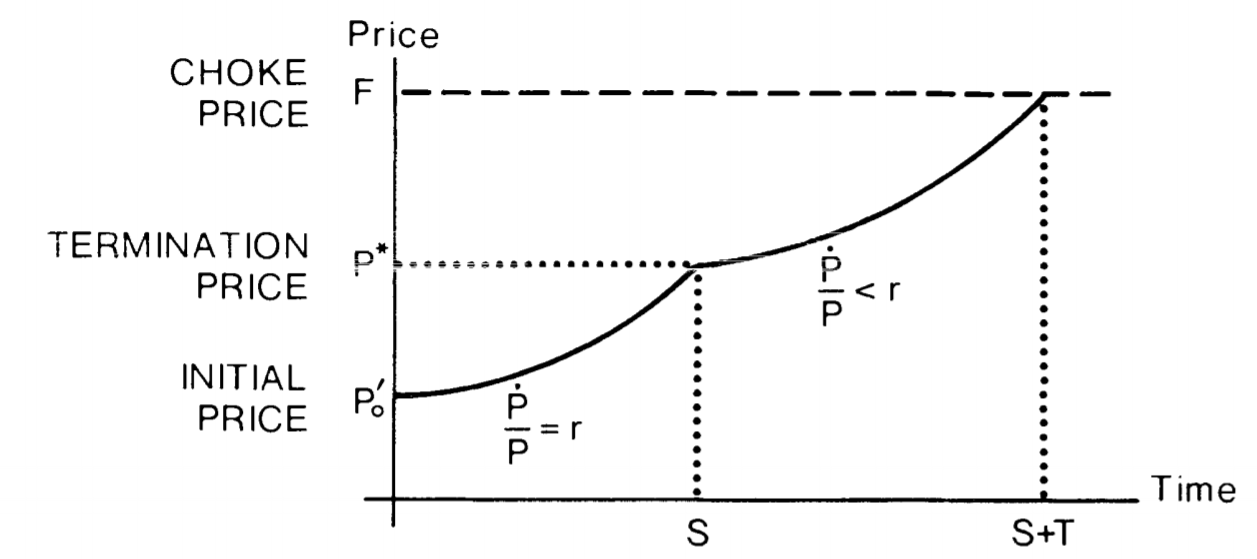
\includegraphics[width=14cm]{template_latex/Pictures/Nash.png}
\centering
\caption{Price path for the cartel model (\cite{salant1976exhaustible})}
\label{nash1}
\end{figure}

Figure \ref{nash1} shows the price path for the market where both the cartel and the competitors exist. Before the cartel starts to form, there are only small extractors existing in the market. Path A in Figure \ref{nash2} shows how the price changes over time during this period. The price will keep growing at the rate of interest until the oil is sold out. Path B is the same as shown in Figure \ref{nash2} where the cartel starts to form. As the world inventory stays the same, the two price paths must cross. The initial price for path A is lower than path B to cross with each other. The formation of the cartel benefits each extractor in the market as it rises the price of the products. The competitive sector can even benefit more than the cartel as they can enjoy the price increase without adjusting their sales. If all the competitive fringe join the cartel, the monopoly market starts to form. As is shown as path C, path C must cross both A and B. Path B contains both A and B in its two phases, it is viewed as an intermediate model between the extremes. If the marginal cost is increasing, the cartel is able to extract the oil for a low cost, however the equilibrium price path will share the same characteristics with the path with a constant marginal cost.
\begin{figure}[h]
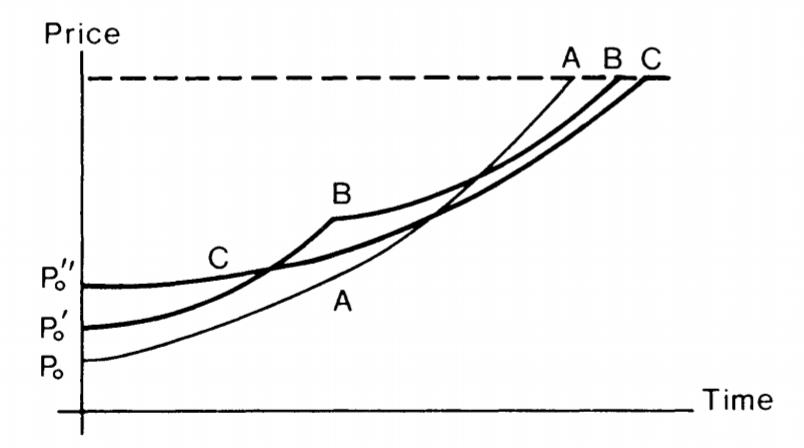
\includegraphics[width=10cm]{template_latex/Pictures/Nash3path.png}
\centering
\caption{3 paths for different market structures (\cite{salant1976exhaustible})}
\label{nash2}
\end{figure}


\subsubsection{Stackelberg Model}
This model is a detailed application of the Nash-Cournot model  where OPEC plays the role of Stackelberg leader. It is divided into two parts, one is OPEC and the other competitive fringe. In the Stackelberg model, OPEC will decide the future oil prices to maximize their profit, while the other competitive fringe will take the price as given. The cartel need to consider its price policy carefully about how the other parts of the market will respond to the policy.

The price path of the Stackelberg model contains both exogenous and endogenous analysis. The exogenous analyses how the residual demand will change under the price given by the cartel. They find the discount rate, which is synonymous with interest rate, is more important than the other parameters. The low interest rate will cause the oil producers to produce the oil slowly, then the residual demand for OPEC is relatively high. In the endogenous analysis, it compares the price paths of minimum cartel and maximum cartel. It reveals that the cartel behaviour will increase the oil price compared with a perfect competitive market. As is shown in Figure \ref{stackel}, when the discount rate equals 2\%, the price path of the maximum cartel is above the price path of minimum cartel (\cite{marshalla1986future}).

\begin{figure}[h]
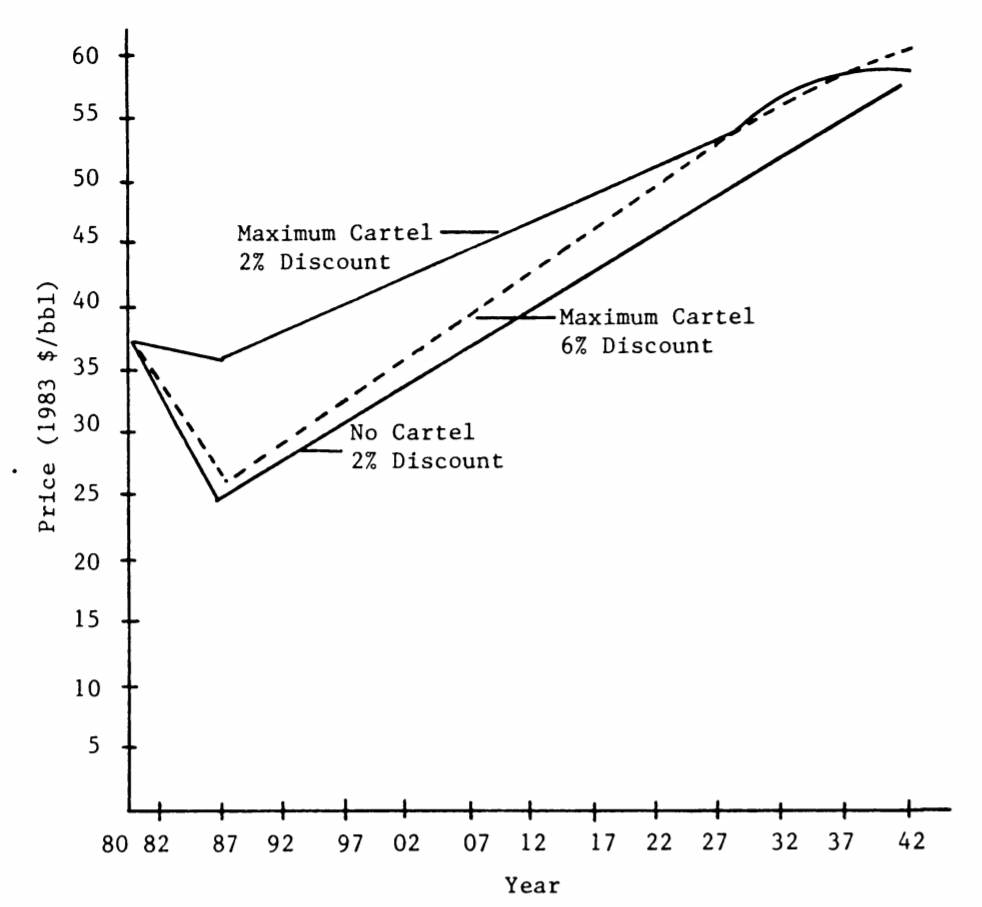
\includegraphics[width=9cm]{template_latex/Pictures/Stackelberg.png}
\centering
\caption{Price path for different discount rate and cartel (\cite{marshalla1986future})}
\label{stackel}
\end{figure}


\subsubsection{Numerical Partial Equilibrium Model}
In 2012, \cite{huppmann2012crude} want to explore OPEC's the market power in recent years. The proposed numerical partial equilibrium model allows for both Nash-Cournot and Stackelberg behaviour in the market. In their model, at least two agents want to maximize their profits under different game theories. They added multiple pool markets to eliminate the spatial price discrimination from the oil suppliers' side. The production cost will be affected by the oil's quality such as API gravity and Sulphur content. Then the oil price is determined by pool price and the transportation cost which refers to the Baltic Dry Index (BDI). Finally, the existence of the arbitrageur will result in the final price as the equilibrium price. The demand for the oil is decided by the linear inverse demand function, so as the oil price increase, the consumer's demand for the oil will decrease as well as the demand other alternative energy resource will increase. The setting of the market power has 5 scenarios. First is the perfectly competitive which indicates no producers has the market power and second is Cournot. The third considers only OPEC has the market power and acts as the dominant supplier, so the remaining oil producers has to compete. The fourth sets Saudi Arabia as the Stackelberg leader while the other OPEC countries did not cooperate inside the OPEC, the other oil producers acts competitively. In the last scenario, the OPEC realize the Cournot market power and form a Cartel inside the OPEC and the other producers has to compete for the remaining market share. As these are related to the optimization part, so we will put weight on exploring the result. The resulted simulation prices over a period from 2005 to 2009. Compared with the real world price, the perfectly competitive formed the lowest price and the Cartel reaches the highest price level. From 2005 to 2007, the real-world price trend was almost as the same as the Stackelberg scenario. Later the real-world price went lower than the Stackelberg but still higher than the perfect competition which indicates the OPEC's market power was reduced since then. In conclusion, from 2005-2007 the Saudi Arabia acted as the Stackelberg leader. The OPEC countries did not cooperate for maximize their profit as Cartel while resulted in the Cournot competition. The other suppliers outside the OPEC act as a competitive fringe. After 2007 the price was going close to the prefect competition price level. This reflected the market structure was changing. One explanation to the situation is that the sharp price fluctuation after 2007 influenced suppliers' judgment on the oil market and meanwhile the burst of the oil price bubble added pressure on the oil producers who depends heavily on the oil revenue. To maintain the income target, they had to increase the oil output which enables the market shifting to the prefect competition scenario.

In 2012, (\cite{huppmann2012crude}) want to explore OPEC's the market power in recent years. They used a numerical simulation model to compute the equilibrium prices under the given strategy scenarios. And then compared it with the real price to find which strategy is close to the real-world situation. In their model, at least two agents want to maximize their profits under different game theories. They added multiple pool markets to eliminate the spatial price discrimination from the oil suppliers' side. The production cost will be affected by the oil's quality such as API gravity and Sulphur content. Then the oil price is determined by pool price and the transportation cost which refers to the Baltic Dry Index (BDI). Finally, the existence of the arbitrageur will result in the final price as the equilibrium price. The demand for the oil is decided by the linear inverse demand function, so as the oil price increase, the consumer's demand for the oil will decrease as well as the demand other alternative energy resource will increase. The setting of the market power has 5 scenarios. First is the perfectly competitive which indicates no producers has the market power and second is Cournot. The third considers only OPEC has the market power and acts as the dominant supplier, so the remaining oil producers has to compete. The fourth sets Saudi Arabia as the Stackelberg leader while the other OPEC countries did not cooperate inside the OPEC, the other oil producers acts competitively. In the last scenario, the OPEC realize the Cournot market power and form a Cartel inside the OPEC and the other producers has to compete for the remaining market share. The resulted simulation prices over a period from 2005 to 2009 as the Figure \ref{huppmann2012crude} demostated.

\begin{figure}[h]
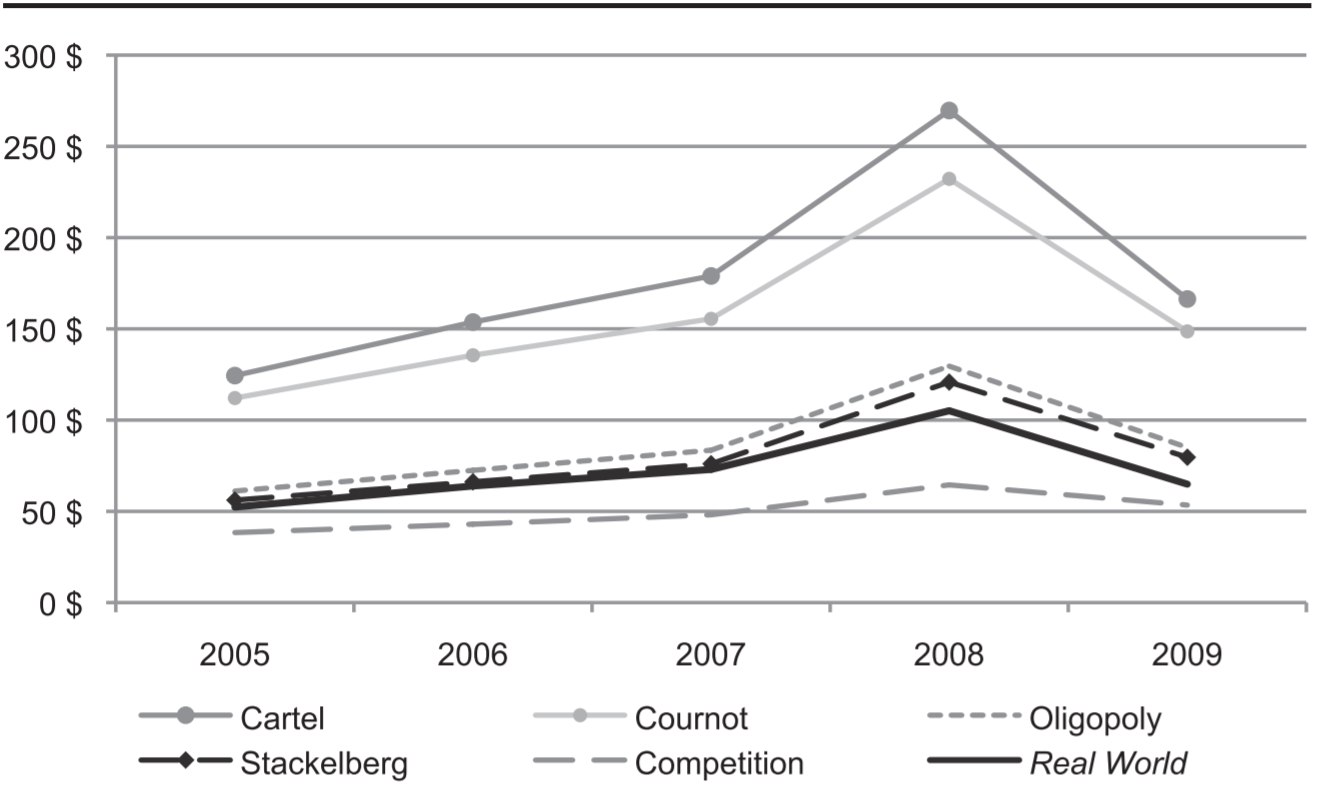
\includegraphics[width=10cm]{template_latex/Pictures/Numerical.png}
\centering
\caption{Simulated price path under different market structures (\cite{huppmann2012crude})}
\label{huppmann2012crude}
\end{figure}

Compared with the real world price, the perfectly competitive formed the lowest price and the Cartel reaches the highest price level. From 2005 to 2007, the real-world price trend was almost as the same as the Stackelberg scenario. Later the real-world price went lower than the Stackelberg but still higher than the perfect competition which indicates the OPEC's market power was reduced since then. In conclusion, from 2005-2007 the Saudi Arabia acted as the Stackelberg leader. The OPEC countries did not cooperate for maximize their profit as Cartel while resulted in the Cournot competition. The other suppliers outside the OPEC act as a competitive fringe. After 2007 the price was going close to the prefect competition price level. This reflected the market structure was changing. One explanation to the situation is that the sharp price fluctuation after 2007 influenced suppliers' judgment on the oil market and meanwhile the burst of the oil price bubble added pressure on the oil producers who depends heavily on the oil revenue. To maintain the income target, they had to increase the oil output which enables the market shifting to the prefect competition scenario.

\subsection{Optimization models}

Optimization models are depended on which sectors optimize. Understanding the value movement of oil is extremely chaotic and complicated. An impact of non-linearity regarding utilization capacity by OPEC or a part of OPEC and condition of the long-term market as an explanatory variable. Moreover, the existence of non-linearity between OPEC spare capacity and the oil value of long-run markets also accounts for adjustment in real oil prices. Some Result indicates that not any single factor plays a vital role within the price fluctuation and even small impact directly effect on economic development. During this section, we are targeting various techniques of an optimization model which is widely used from 1970. Within the past few years, there's plenty of research to research the oil demand decreases from OPEC or Non-OPEC countries. But the worth of oil still increases.\\ 

The optimization model offered a very structured framework to know market power that sort of approach was widely applied for the event of the energy system model (\cite{hogan1975energy}) and a few specific sorts of models (\cite{salant1982imperfect}). However, there's a lot of limitations in their application (\cite{huppmann2012crude}). Optimization approaches deliver information within the sort of data and objective function. The modeling process identifies optimal solutions on a predefined goal, and there are not any robust approaches for large-scale applications (\cite{lund2017simulation}).\\

In the literature, review the author describes how an agent likes Saudi Arabia being one agent with the market power solves the optimization in its favor. In some models, OPEC and an element of OPEC are taken under consideration to be the one agent who optimizes its strategy. That sort of path incredibly uses full for economic incentives and profit maximization. But it's extremely limited ability to predict actual market outcomes (\cite{huntington2013oil}).\\ 


Some optimization technique isn't bear in mind to be an optimization model in this paper. The rationale is when price rise in \cite{deam1973world} develop a model on the idea of guessed competitive market. His approach is incredibly simple he considers the short-term price is a weighted average of marginal costs, and therefore the long-term price is found by solving linear program that minimizes that cost (extraction, refinery, and transportation) to consumers. These type models producing for the lowest cost that why they didn't recognize as an optimization model. In keeping with author individual producer cannot influence the price (\cite{huntington2013oil}).\\ 

\cite{kalymon1975economic} developed an inter-temporal model, which is predicated on the efficient allocation of energy resources employing a depletable resource theory. Within the OPEC higher cognitive operation policy few things are missing like bound on price and also the source of energy, which is about backstop technology. When OPEC faces an inter-temporal optimization problem. \cite{kalymon1975economic} build several models to explore OPEC behavior from the event of two different strategies. In his first framework, one agent like the Kingdom of Saudi Arabia and Iran acting become a residual producer and other he simulate the model to grasp different market sharing structures utilized by OPEC. He finds an awfully interesting result when the optimal price for OPEC is sensitive to the prospect cost of capital relies upon importing country and second when the optimal price isn't very sensitive. due to total reserve size or the expansion rate of the domestic market .\\

In 1976. Two different models employed by the oil market, the primary one is that the model proposed by \cite{ben1976oil}. Which is relied on monopolist designs making policy utilized by OPEC for the long term outcome and supply from non-OPEC producer simulate by simple calculation of price rule. The Second model is developed by \cite{ezzati1976future}, this model is based on applied linear programming optimization and macroeconomic framework. This strategy relies on the weighted sum of OPEC member utilities in the World energy market. the objective of this model is to estimate important factor (production and consumption) using functions of constant-elasticity and discrete approximation of these function used by the linear program.\\

\cite{daly1982recent} proposed approach which is about the different goals for OPEC member community. In this model demand of economic activity is a log-linear function and thought of lag distribution on the previous oil price is relative to other goods. Daly et al. measure OPEC cartel stability by using the ratio of market shares and production reserves. This model actually projected future paths for production and reach target revenue fallowed by price maximizes. but this model didn't address the one stable value of price give by current behavior.\\


In \cite{celta2000opec} a model employed by OPEC, which is truly supported maximizing the financial aid of OPEC rather than maximizing profit. From this model, they conclude OPEC countries should define the domestic oil price adequate the marginal revenues from the oil export market.\\

\cite{horn2004opec} developed a simple and transparent strategy on the basis of the numerical value assumption. In this model, he just set an upper limit for the production of Non-OPEC community because of the calculation of geologic constrains. In his approach work two different ways: the first way he simulates past data as a depletable resource per the Hubbert curve. The second one uses Gompertz function with the data set. that is allowed to set the upper limit or asymptote. In his approaches, he has looked for a group of costs to maximize OPEC surplus. \\

\cite{huppmann2012crude} discussed how effective way observed of oil price in numerous global regions and proposed approach with the mix of a hub and spoke model. He doesn't consider any true optimization technique in his proposed model, he introduced the global oil market in additional than one pool. However, the supplier has the liberty to settle on any consumer directly, and only the amounts purchased and sold by the arbitragers are routed via the pool hubs, unlike within the hub and spoke approach. He's thinking this can be the most effective strategy to know the convergence price movement of a special region. In step with his approach, there's two exemption within the optimization model. A model develops by \cite{al2008model} and FRISBEE Model. He also considered how Saudi Arabian company Saudi Aramco increase profit by reducing supply. However, the full strategic decision not taken other members of the OPEC community.

\subsection{Simulation models}
According to Powell, he summarized the existing world oil market models and divided them into the inter-temporal optimization model and behavioral simulation models (\cite{powell1990target}). For the oil producer, the former model describes these producers' actions are economically rational and they forecast their maximum benefits like profits, utility, or market share in the future. While the later model puts the producers into a situation that they have limited information, calculating resource and the assumption. They have to make decisions based on current or historical data or the rules of thumb. Also, the simulation model can be utilized to predict agents' behavior under given a set of conditions \cite{wurbs1993reservoir}. Compared with the optimization model, the simulation model could yield a more plausible behavioral assumption towards the oil producers' behavior as they do not have sufficient knowledge of the future so the supply-demand equilibrium will affect the price.

Huntington etal. proposed that the behavior rules in simulation models could be classified in three approaches: strategy selection, econometric fit and rule of thumb (\cite{huntington2013oil}). In strategy selection, where different behavior rules were simulated for the oil producer to find which one is the most beneficial rule. Econometric fit approach uses econometric model and historical data to find key parameter affecting the oil market and related behavior which fits each agent. Last approach is based on the rule of thumb as taking the capacity utilization or the target price zone into consideration to describe the oil producers' behavior. As some models follow at least one approach, so this part will review on some simulation models without classifying.

In 1975, a dynamic simulation model was proposed by Blitzer et al. (\cite{blitzer1975dynamic}), which tests 6 policy options related to the oil price and output that OPEC may apply on their export decision. Then these options were ranked on various assumptions such as the rate of growth of domestic absorption of oil earnings within OPEC, the rate of oil production expansion capacity, the response ability towards the variation on the investment in alternative energy when oil price changes, and the growth rate of the world energy demand. In conclusion, the alternative energy sources of OPEC's Oil are influenced by the OPEC's oil price. As the result of price competition, a large amount of the alternatives of OPEC oil will not come out if the oil price remains a low price level for long term. Meanwhile, the long-term expected OPEC oil price is the key parameter for future oil price prediction as well as the standard for oil import countries to find the alternatives of the OPEC's oil.


In 1988, a recursive simulation model was developed by Baldwin and Prosser for the World Oil Market (WOM) (\cite{baldwin1988world}). Both demand and supply functions in the model are dynamic, and the three participators are oil consumers, non-OPEC oil producers and OPEC. For the oil consumers, they want to maximum their benefits in terms of their expenditure on the oil and non-OPEC oil producers expect to maximize their profit. OPEC decides the price or the output depends on the market situation so that non-OPEC oil producers and consumers will be the price takers. Two setting are used for simulate the OPEC's strategy. OPEC uses the price response function to set prices to achieve the best level of capacity utilization, or to limit output by following the rules of demand and supply to achieve a balanced oil price and market. Subsequently, the results show that OPEC can learn to adjust the supply and demand and maintain a balance between the oil price and its output.


In regard to know whether the OPEC will raise their oil output largely in 20 years as the U.S. Department of Energy predicted. In 2004, Gately used a simulation model to compare the payoffs resulted by the faster and slower oil output growth \cite{gately2004opec}. The model takes the conditions as the OPEC's response towards the price fluctuation, predicted market share as well as the related export profit, and the countries' choices inside the OPEC with regard to the faster or lower output growth into consideration. And the result turned out that there would be not so much difference between two scenarios, the growth of the output will not bring more profit as the oil price will going down. From a comprehensive perspective, it is in the interest of OPEC to maintain a reasonable growth rate.


\section{Reduced form models}
The advantage of the structural model and the calculation model is that when it is used to analyze each case can analyze in detail the various factors that lead to the long-term fluctuation of international oil prices. But not every scientific research in every situation will pay close attention to market behavior. Sometimes, scientists only care about price movements over a period of time. The calculation model and the structural model are overly dependent on too many model parameters, which means that when these parameters are wrong, the calculation effect of the entire model will be greatly reduced (\cite{huntington2013oil}). Therefore, the reduced form model is very suitable for studying the statistical relationship between changes in oil prices and changes over time and other related variables. The reduced form model can be a powerful help for analysts in predicting short-term changes in future oil prices. Reduced form model is usually divided into linear time series model and nonlinear time series model. In this chapter, we will introduce two of the most popular analysis models, namely, Vector Autoregression Model (VAR) Structural Vector Autoregression Model (SVAR).

\subsection{Vector Autoregression Model(VAR)}
In 2020, oil prices fell below zero for the first time in history, which not only impacted the entire industry. It also breaks the model that many traders use to calculate risk. For the largest banks on Wall Street, this means that in a short period of time they have to frantically recalculate the value and risk of their trading accounts to account for the possibility that oil prices may become negative. The impact is huge. Considering that the price may drop below zero, banks and traders face potentially significant losses, and at the same time, it also exacerbates severe market volatility. If the bank cannot compile risk indicators correctly, this will be a big trouble.  Of particular concern are put options, which banks usually sell to oil producers to hedge against the risk of a sharp drop in oil prices.  Traditional methods of calculating option prices, such as the well-known Black-Scholes model (\cite{lauterbach1990pricing}), are based on the assumption that oil prices cannot fall below zero. For example, if a bank sells a put option that gives its client the right to sell oil at a price of 20 USD per barrel, it will be confident that it will not lose more than 20 USD per barrel in the transaction. Now, this assumption must be overturned. As the decline in oil prices may be unlimited, there is no longer an upper limit on potential losses. Therefore, in the prediction of international oil prices, it is very important to use a more reasonable model. The VAR model is a statistical indicator used by many banks and trading institutions to estimate the probability of loss. Due to the impact of oil prices becoming negative, the VAR model will be worsened. More and more widely used.

The VAR model is an unstructured model. When we want to use a structured model to describe the dynamic relationship between variables, a complex economic theoretical foundation is indispensable. In the process of analysis, we can find that the lag period will affect the current period. When this method is applied to some complex systems, it will be found that its feasibility is greatly reduced.  In the process of model structuring, endogenous variables can appear at both ends of the equation at the same time, which makes parameter estimation and model inference very complicated. This method of structuring the model completes the expansion of a univariate auto-regressive model to an auto-regressive model composed of multiple time series variable vectors.  In the modeling and estimation of oil prices, the VAR model exerts great reliability and applicability. The price of oil is affected by some specific factors and has a strong correlation with many macroeconomic variables. The macroeconomic variables mentioned here mainly refer to natural gas prices, gold prices or stock prices. VAR model is usually used to analyze the changes and interdependencies between multiple time series (\cite{huntington2013oil}).
The reduced form of k variables expressed as VAR(p), the unrestricted p-order VAR model is given by: 

\[y_{t}=c+B_{1} y_{t-1}+B_{2} y_{t-2}+\cdots+B_{p} y_{t-p}+e_{t}\] 

where y means a $k*1$ vector of the variable of interest, $c$ is the constant a $kx1$ vector (intercept), $B$ is a $k*k$ matrix(for each i = 1,2,3,..,p ) and the $e_{t}$ is a $k*1$ vector of error items (\cite{huntington2013oil}). So, the model can also be described as: 
\[y_{t}=c+B(L) y_{t-1}+e_{t}\]
Where $L$ is the lag operator and $B(L)$ is a polynomial function (\cite{huntington2013oil}). 

The main features of the VAR model are: 1.The value of parameters in the VAR model can be zero. 2.The VR model does not contain any explanatory variables that are current variables. 3.The VAR model requires a lot of parameter estimation. 4.The unconstrained VAR model can be widely used to forecast oil prices.
The VAR model can be widely used in time series analysis. Relative to general time series models, VAR allows contemporaneous correlation and feedback effect. VAR model is convenient for interval estimation, error analysis and model diagnosis. VAR can describe the mutual influence between variables. By using VAR model can get more accurate results about the dynamic linear correlation

\subsection{Structural Vector Autoregression Model(SVAR)}
The world crude oil price is the result of the interaction between supply and demand, and the lagging effect is obvious. Then, when considering the combined effects of both the lag period and the current period, the VAR model obviously has shortcomings. The SVAR model can effectively solve this problem, clarify the current relationship between crude oil demand and supply and the potential for the variables in the model. The relationship has been explored in more depth to make up for the shortcomings of the VAR model. Sims(\cite{}) transformed VAR from a purely statistical model into a general framework that can identify dynamic relationships between economic variables through economic models, thus creating a macro-econometric method that is different from the traditional simultaneous equations. Bernanke (1986) and Sims (1986) put forward the structural vector auto-regressive model (SVAR) on the normal traditional VAR model, adding the current influence of variables. The SVAR model is the structural formula of the VAR model, that is, the model contains the inter-variable  Current relationship. Killian (2009) used the structural VAR framework to distinguish oil price shocks among oil supply shocks, aggregate demand shocks and preventive demand shocks, and found that oil price increases were mainly driven by demand(\cite{kilian2009not}).

An SVAR model is usually executed in the following four steps. 

Step 1 is to establish many different structural equations based on economic theory, such as the function of oil production and price, or the function of oil demand and supply. Taking the latter as an example, the following equation can be established.

\[A(L) y_{t}=c+w_{t}\]

Where $y_{t}$ stands for the variables like, price quantity and so on. The $w_{t}$ means the structural shock, like the demand shock or the supply shock (\cite{huntington2013oil}).
Step 2: According to economic theory, establish a one-to-one mapping relationship between reduced form parameters and structural parameters. In order to achieve this goal, the reduced form VAR model needs to be estimated, and some variables in the structural equation need to be excluded to achieve its limitations. For example, when researchers want to accurately analyze the supply of oil, factors such as national income, stock market conditions, and the development of oil-using industries will not be considered. When analyzing the demand function, the production cost of oil, the total oil reserves and other variables related to the supply function will not be considered. Step 3 is to get the conclusions from the structural parameters (\cite{huntington2013oil}).  

In addition to adding exclusive restrictions to structural equations, there are many other methods to obtain the potential relationship between the variables of the model, such as sign restrictions. Killian and murphy (\cite{kilian2014role}) proposed a very efficient SVAR model in the article. 

In their article, based on economic theory and other external information, they combined the implied price elasticity limits of oil demand and oil supply with symbolic restrictions, and established an SVAR model. They proposed four identifying restrictions. They are oil production, real activity, real price of oil and inventories (\cite{kilian2014role}). However, they found that only sigh restrictions cannot fully obtain the relationship between oil demand and supply shocks. Therefore, other restrictive factors must be imposed. Firstly, impose restrictions on the price elasticity of oil supply. But this restriction does not limit the level of impulse response, but only limits its relative size. In their SVAR model, a limit of 0.025 is imposed on the price elasticity of the impact of oil supply. The specific value of the limit is not unique. Users can increase the limit value by increasing the number of allowable models. The resulting posterior distribution diagram is almost the same as the posterior distribution diagram when the limit value is 0.025 (\cite{kilian2014role}). Secondly, limit the price elasticity of oil demand. The price elasticity of oil demand is related to the shock response of oil production, the actual price of oil, and the rate of unexpected supply interruptions. The author limits the demand elasticity in use to zero, and through a series of surveys and studies, referring to factors such as US household survey data, set 0.8 as the long-term price elasticity estimate (\cite{kilian2014role}). Thirdly, apply dynamic sign restriction. In addition to the two restrictions mentioned above, dynamic sigh restriction will be added eventually. It involves the dynamic response of oil prices when the flow supply is unconventionally interrupted. This additional restriction is necessary.  The restriction imposed by the authors is that the response of the actual price of oil to shocks must be positive for at least 12 months (\cite{kilian2014role}). Due to oil supply problems, the oil supply was interrupted, which led to a decline in inventories. The response of oil production activities and actual economic activities to this interruption is negative, and correspondingly, the response of actual oil prices must be positive.  At the same time, due to the uncertainties in the changes in oil demand, the author did not impose any dynamic sign restriction on the shock of oil demand.



\section{Artificial intelligence models}
Energy and financial markets are emerging fields of artificial intelligence applications. At present, artificial intelligence models are one of the tools commonly used in oil price prediction. The artificial intelligence model provides the ability to recognize complex patterns, automated reasoning. It also can make decision based on data. Compared with traditional modeling methods that require the use of parametric methods to build models, artificial intelligence models are not subject to predefined constraints. It provides an inductive solution to the problem rather than a regression method, and finds existing patterns in the data. The most common artificial intelligence models are artificial neural networks, deep learning, machine learning, genetic algorithms, support vector machines, fuzzy logic, and so on.

\subsection{Artificial neural network Models}
The main purpose of the artificial neural network (ANN) is to establish a complex mapping between goals and influencing factors and parameters. It can be defined as a parallel processing model of biological neuron structure. Each ANN usually consists of many connected nodes or neurons. It includes an input layer, one or more hidden layers and an output layer (\cite{Y3}). The number of nodes depends on the network architecture chosen. It also depends on the number of input and output variables required. The input layer has the same number of nodes as the independent variable. The output layer has the same number of nodes as the dependent variable. Each input is modified by the weight like the figure \ref{y1}.

\begin{figure}[h]
    \centering
    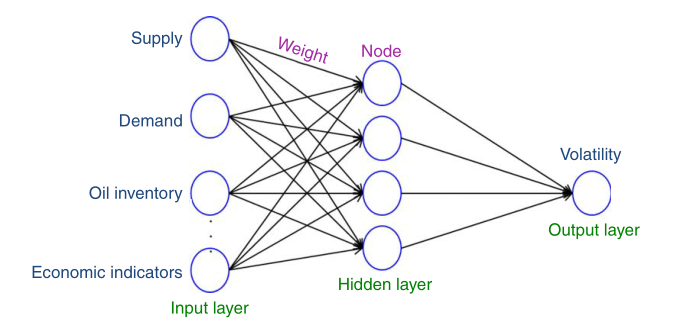
\includegraphics[width=0.6\textwidth]{template_latex/Pictures/y1.png}
    \caption{Three-layer artificial neural network structure (\cite{Y3})}
    \label{y1}
\end{figure}
Oil market volatility modeling uses the value of the target variable to predict oil price volatility over time. The input variables can include crude oil prices, supply, demand, spare capacity, and economic indicators (\cite{Y2}).


\subsubsection{Objective determination}
In objective determination stage, data collection and preparation are the most important and time-consuming. The difficulty is mainly to determine the frequency and size of the data (\cite{Y4}). For short-term forecasts, high-frequency data is preferred, like daily data. However, the purchase cost of these data is high. In addition, weekly and monthly data are also the first choice for other forecast ranges. Another influencing factor is the data size. Generally speaking, the optimal amount of data required to develop an ANN model is often very complicated. The more data points, the better the network generation. From the experience of some literature, the data points in the network should be at least 10 times that of the connection (\cite{Y5}). This problem is called the "curse of dimensionality" (\cite{Y2}). This is not the case when dealing with economic time series. As economic conditions change over time, old information may have a negative impact on the prediction results, resulting in poor generalization of the model (\cite{Y4}).

\subsubsection{Data pre-processing}

ANN is better used for normally distributed data and non-seasonal data. If the input shows a trend or periodic changes, the conversion is required. This form of conversion includes the variable first derivative, relative variable difference, natural logarithm of relative variable, square root of variable, and trigonometric functions (\cite{Y2}).

Normalization is to control the value range of input data within the standard area. Normalization is generally used to prevent larger values from overwriting smaller values that are equally important. Normally, the mean or standard deviation normalization method is used to normalization.
\begin{figure}[h]
    \centering
    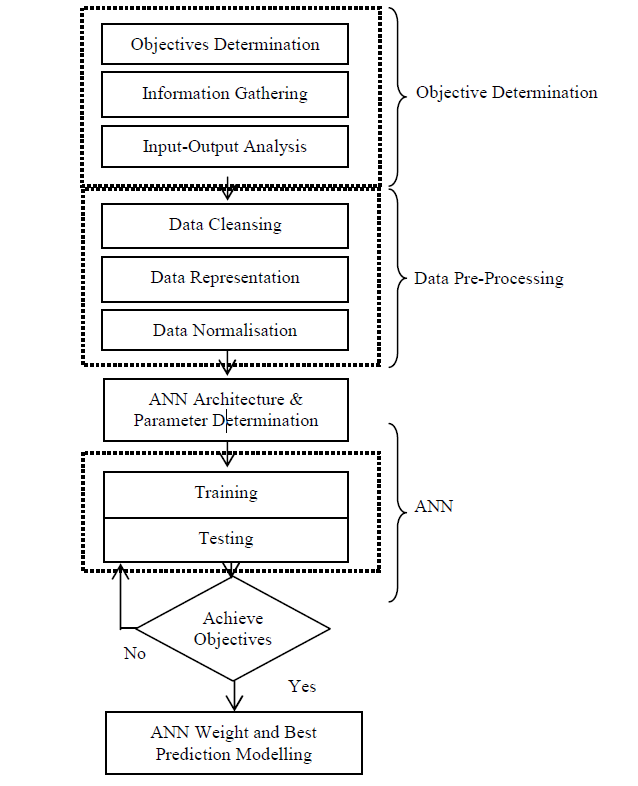
\includegraphics[width=0.6\textwidth]{template_latex/Pictures/y2.png}
    \caption{Flowchart of ANN design (\cite{Y1})}
    \label{y2}
\end{figure}
\subsubsection{Model design}
Choosing a network structure is one of the first tasks for building a neural network. There are two types of network structures that are often used: recurrent network (Elman) and multi-layer feed-forward network.

The activation function acts on the value returned by the input function and introduces non-linearity into the neural network to enrich the representation ability of the neural network. In the hidden layer, the most widely used activation functions for finance are sigmoid functions and symmetrical sigmoid functions. The threshold behavior of the sigmoid function describes most financial sequences. However, the recent trend in financial applications is toward a symmetrical sigmoid function (\cite{Y6}).

\subsubsection{Training and testing}
During the training process, the network iterates repeatedly until it can output the error threshold. Usually, the training data subset needs to go through dozens to hundreds of iterations. During the training process, it does not participate in the adjustment of weights and thresholds, but will continue to use validation data to test the performance of the network. When the error of the validation data stops decreasing or starts to increase, the training is stopped. Because if the training is not restricted, the neural network will over-learn or over-fit the training data, and the performance of the new data set may be poor.


\subsubsection{Summary}
Artificial neural network is a powerful tool to predict future oil prices based on past oil prices. Mahdi et al studied three different neural network models, Multi-layered Perceptron (MLP), Functional Link Neural Network (FLNN) and Self-Organized MLP (SoMLP) for the oil price (\cite{Y7}). They compared the 10 Performance on each data set, the results show that the neural network performs better when it is stationary. Based on the characteristics of ANN, combining ANN with other methods can overcome some problems of ANN to improve prediction performance.

\chapter{Discussion}

\section{Structural models}

\subsection{Game-theoretic equilibrium models}
Game theoretic-equilibrium models study the dominating players of the oil market and provide price paths of simulations under several ideal market structures. These models help us to better understand the agents of the markets and their behaviours. However, in recent years, the rise of shale oil has exerted more power in the crude oil market. The equilibrium of the market seems to shift to an other stage. Whether OPEC can still lead the market remains a problem(\cite{ansari2017opec}). As the real oil market is a complex one, it contains more agents than the equilibrium models have.  The models need more computational power when dealing with large volumes of data, in which case, the computational models will take over.

\subsection{Optimization models}
Based on the structure of the optimization model we are able to easily think there are numerous practical challenges to objectify future prices. It's doesn't matter we've got an sufficient amount of information and accurate objective functions. There's uncertainty related element within the development of technological future fuel price fluctuations are typically considered as matters of risk and uncertainties which will be addressed in quantitative risk assessments and sensitivity analyses (\cite{lund2017simulation}). But In some case's optimization model have a really powerful tool to grasp the accurate description of this energy system.

\subsection{Simulation models}
Simulation model takes multiple key factors into consideration and generates various alternative solutions for analyzing and comparing. As the user could use simulation model to calculate and test the resulted performances by combing arbitrarily chosen elements such as cost, budget, market share, and others. It gives users the power and grounds for decision-making (\cite{lund2017simulation}). The limitation in the simulation model is that the model depends more on the empirical evidence rather than economical theory so that the performance of agents' performance and the expected goal may not be reached. Although it demonstrated that agents' behavior might be plausible rather than the optimal.


\section{Reduced form models}
By the research and analysis of the two most widely used and popular reduced-form models. We found that the reduced-form model can effectively solve the parameter dependence problem. Compared with the structural model and the calculation model, the reduced form model has a huge advantage in this regard. At the same time, the reduced-form model can analyze the data more intuitively, and can obtain the relationship between certain variables more quickly. And when we are studying a complex economic process and human behavior, we do not need a lot of model estimation assumptions. However, because the operating mechanism of many reduced-form models, including the VAR model, treats the complex economic process and human behavior as a "black box" as a whole, so they cannot live up to the specific realization mechanism of this set of causality.  Therefore, the use of the SVAR model is a good supplement to this shortcoming and can obtain the relationship between variables.

\section{Artificial intelligence models}
Compared with traditional regression techniques, the advantage of artificial neural networks is that they can solve highly nonlinear complex dynamic problems and does not to know the relationship between the input and output variables in advance. Secondly, it can process continuous data as output or input.

But it also has its problems. The selection and processing of the data set is very complicated, and the accuracy and dimension of the data set are very high. And it failed to generate profits while using non-stationary data. Over-fitting and other issues may also occur during training

\include{Chapters/chapter_5}

\printbibliography[
title={Bibliography}]





%% Backmatter
\backmatter
%%%%
%%% Danksagung
%%%

\thispagestyle{empty}
\chapter*{Danksagung}

Danke!\\
Wähle deine Sprache selber! Die Erklärung der Verfasserin bitte immer in DEUTSCH!
Ließ bitte das Dokument Formatvorlage.doc (ee2.biz - Lehre - Vorlagen) gründlich durch, auch wenn du in \LaTeX  schreibst!
\\[1cm]
%
Maxine Somebody, im Oktober 2010		% optional

%\include{Chapters/Erklaerung1} 	

%%%
%%% Erklärung bei Gruppenarbeit
%%%

\thispagestyle{empty}
\chapter*{Erkl\"{a}rung der Verfasserin}

%
Hiermit erkl\"{a}re ich eidesstattlich, dass ich die vorliegende Arbeit
selbstst\"{a}ndig und ohne Benutzung anderer als der angegeben Hilfsmittel angefertigt habe, sowie die 
aus fremden Quellen direkt oder indirekt \"{u}bernommenen Gedanken als solche kenntlich gemacht habe.
\\
Die Arbeit wurde bisher in gleicher oder \"{a}hnlicher Form keiner anderen Pr\"{u}fungsbeh\"{o}rde vorgelet 
und auch  noch nicht ver\"{o}ffentlicht.%
\\[2cm]
%
\begin{multicols}{2}

Dresden, 31. Juli 2020
\\[2cm]
Group member 2 Yu Kong
\\[2cm]
Group member 4 Dongxin Guo

\columnbreak

Group member 1 Yushan Yang
\\[2cm]
Group member 3 Xiao Cui
\\[2cm]
Group member 5 Anurag Trivedi

\end{multicols}	% for group work


\end{document}

